\documentclass[tikz, border=5mm]{standalone}
\usetikzlibrary{calc, arrows.meta, positioning, matrix}

% Macros de Geometría
\newcommand{\defNodes}[1]{
    \coordinate (#1_1) at (0.8, 1.2);   \coordinate (#1_2) at (0.5, 2.8);
    \coordinate (#1_3) at (2.2, 0.6);   \coordinate (#1_4) at (2.6, 2.1);
    \coordinate (#1_5) at (1.5, 4.2);   \coordinate (#1_6) at (3.8, 1.4);
    \coordinate (#1_7) at (4.2, 3.2);   \coordinate (#1_8) at (2.5, 5.5);
    \coordinate (#1_9) at (1.0, 6.5);   \coordinate (#1_10) at (3.5, 6.8);
    \coordinate (#1_11) at (5.2, 4.5);  \coordinate (#1_12) at (5.8, 2.2);
    \coordinate (#1_13) at (7.2, 1.0);  \coordinate (#1_14) at (7.8, 2.8);
    \coordinate (#1_15) at (6.5, 4.0);  \coordinate (#1_16) at (5.5, 6.5);
    \coordinate (#1_17) at (4.5, 8.2);  \coordinate (#1_18) at (2.2, 8.2);
    \coordinate (#1_19) at (7.2, 5.8);  \coordinate (#1_20) at (8.5, 4.8);
    \coordinate (#1_21) at (7.0, 7.5);  \coordinate (#1_22) at (8.2, 7.2);
    \coordinate (#1_23) at (5.8, 8.8);  \coordinate (#1_24) at (1.8, 3.5);
    \coordinate (#1_25) at (3.2, 0.4);  \coordinate (#1_26) at (4.8, 0.8);
    \coordinate (#1_27) at (0.6, 8.5);  \coordinate (#1_28) at (8.8, 1.2);
    \coordinate (#1_29) at (9.0, 3.5);  \coordinate (#1_30) at (9.2, 6.0);
    \coordinate (#1_31) at (7.5, 8.8);  \coordinate (#1_32) at (8.4, 8.5);
}

% Malla k-NN base
\newcommand{\drawBaseEdges}[1]{
    \draw[base edge] (#1_1)--(#1_2) (#1_1)--(#1_3) (#1_1)--(#1_4) (#1_2)--(#1_5) (#1_2)--(#1_24) (#1_3)--(#1_6) (#1_3)--(#1_25) (#1_4)--(#1_7) (#1_4)--(#1_11) (#1_5)--(#1_9) (#1_5)--(#1_7) (#1_6)--(#1_24) (#1_6)--(#1_26) (#1_7)--(#1_12) (#1_8)--(#1_9) (#1_8)--(#1_10) (#1_8)--(#1_12) (#1_9)--(#1_27) (#1_10)--(#1_17) (#1_10)--(#1_11) (#1_11)--(#1_16) (#1_12)--(#1_13) (#1_13)--(#1_26) (#1_13)--(#1_28) (#1_14)--(#1_15) (#1_14)--(#1_28) (#1_14)--(#1_29) (#1_15)--(#1_19) (#1_15)--(#1_16) (#1_16)--(#1_21) (#1_17)--(#1_18) (#1_17)--(#1_19) (#1_18)--(#1_23) (#1_18)--(#1_27) (#1_19)--(#1_20) (#1_20)--(#1_29) (#1_20)--(#1_30) (#1_21)--(#1_32) (#1_21)--(#1_23) (#1_22)--(#1_30) (#1_22)--(#1_31) (#1_22)--(#1_29) (#1_23)--(#1_31) (#1_24)--(#1_27) (#1_25)--(#1_26) (#1_25)--(#1_28) (#1_30)--(#1_32) (#1_31)--(#1_32);
}

\begin{document}
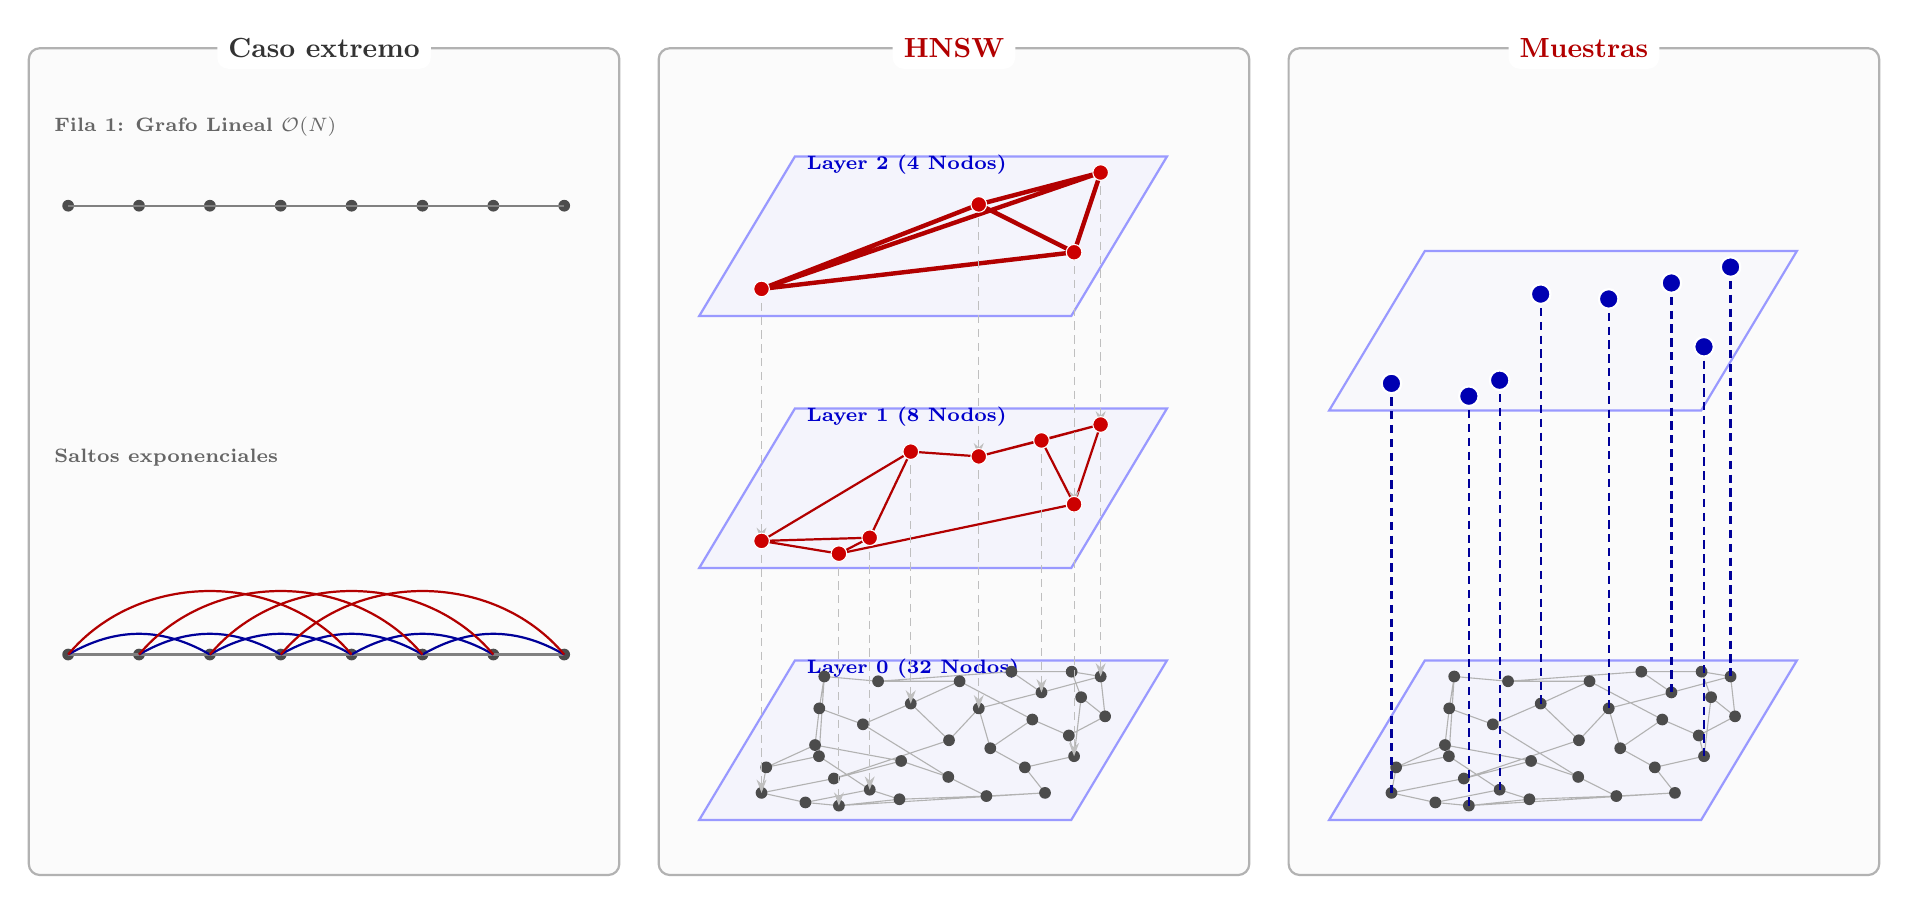
\begin{tikzpicture}[font=\sffamily, panel frame/.style={draw=black!30, fill=gray!3, rounded corners, thick}, panel title/.style={font=\bfseries, align=center, fill=white, inner sep=4pt, rounded corners}, row subtitle/.style={font=\scriptsize\bfseries, color=black!60, anchor=west}, base node/.style={circle, fill=black!70, inner sep=1.5pt}, hnsw node/.style={circle, fill=red!80!black, inner sep=2pt, draw=white}, centroid node/.style={circle, fill=blue!70!black, inner sep=2.5pt, draw=white, thick}, base edge/.style={black!30}, hnsw edge/.style={thick, red!70!black}, jump edge/.style={thick, blue!60!black}, drop edge/.style={->, >=Stealth, densely dashed, black!25}, centroid drop/.style={densely dashed, thick, blue!60!black}, c/.style={draw, minimum width=1.0cm, minimum height=0.5cm, fill=white, outer sep=0pt, anchor=center, font=\scriptsize}, h/.style={c, fill=gray!20}, mat edge/.style={->, >=Stealth, dashed, thick, black!70}, layer plane/.style={draw=blue!40, fill=blue!10, fill opacity=0.3, thick}]

    % =========================================================================
    % CUADRO 1: Evolución 1D
    % =========================================================================
    \begin{scope}[xshift=0cm, yshift=0cm]
        \draw[panel frame] (0, 0) rectangle (7.5, 10.5);
        \node[panel title, text=black!80] at (3.75, 10.5) {Caso extremo};

        % FILA 1: Grafo Lineal (Sin flechas)
        \node[row subtitle] at (0.2, 9.5) {Fila 1: Grafo Lineal $\mathcal{O}(N)$};
        \begin{scope}[yshift=8.5cm]
            \foreach \i in {1,...,8} { \coordinate (R1_\i) at ({0.5 + (\i-1)*0.9}, 0); \node[base node] at (R1_\i) {}; }
            \foreach \i [evaluate=\i as \next using int(\i+1)] in {1,...,7} { \draw[thick, black!50] (R1_\i) -- (R1_\next); }
        \end{scope}

        % FILA 2: Ligas Exponenciales (Sin flechas)
        \node[row subtitle] at (0.2, 5.3) {Saltos exponenciales};
        \begin{scope}[yshift=2.8cm]
            \foreach \i in {1,...,8} { \coordinate (R2_\i) at ({0.5 + (\i-1)*0.9}, 0); \node[base node] at (R2_\i) {}; }
            \foreach \i [evaluate=\i as \next using int(\i+1)] in {1,...,7} { \draw[jump edge, black!50] (R2_\i) -- (R2_\next); }
            \foreach \i [evaluate=\i as \next using int(\i+2)] in {1,...,6} { \draw[jump edge] (R2_\i) to [bend left=30] (R2_\next); }
            \foreach \i [evaluate=\i as \next using int(\i+4)] in {1,...,4} { \draw[jump edge, red!70!black] (R2_\i) to [bend left=50] (R2_\next); }
        \end{scope}

        % FILA 3: Skip List Ajustada
        %%% \node[row subtitle] at (0.2, 3.8) {Fila 3: Skip List Clásica ($\mathcal{O}(\log N)$)};
        %%% % Reducción estricta de escala y márgenes de columna para forzar contención
        %%% \begin{scope}[shift={(3.75, 1.8)}, scale=0.28, transform shape]
        %%%     
        %%%         \matrix (M) [matrix of nodes, column sep=1.5mm, row sep=-\pgflinewidth, anchor=center] {
        %%%             |[h]| (4) & & & & & & & & |[c]| (4) & & & |[h]| (4) \\
        %%%             |[h]| (3) & & & & & |[c]| (3) & & & |[c]| (3) & & |[c]| (3) & |[h]| (3) \\
        %%%             |[h]| (2) & |[c]| (2) & & |[c]| (2) & & |[c]| (2) & & |[c]| (2) & |[c]| (2) & & |[c]| (2) & |[h]| (2) \\
        %%%             |[h]| (1) & |[c]| (1) & |[c]| (1) & |[c]| (1) & |[c]| (1) & |[c]| (1) & |[c]| (1) & |[c]| (1) & |[c]| (1) & |[c]| (1) & |[c]| (1) & |[h]| (1) \\
        %%%             |[h]| (head) & |[c]| a & |[c]| b & |[c]| c & |[c]| d & |[c]| e & |[c]| f & |[c]| g & |[c]| h & |[c]| i & |[c]| j & |[h]| (tail) \\
        %%%         };
        %%%         \begin{scope}[every path/.style={mat edge}]
        %%%             \draw (M-1-1.east) -- (M-1-9.west); \draw (M-1-9.east) -- (M-1-12.west);
        %%%             \draw (M-2-1.east) -- (M-2-6.west); \draw (M-2-6.east) -- (M-2-9.west); \draw (M-2-9.east) -- (M-2-11.west); \draw (M-2-11.east) -- (M-2-12.west);
        %%%             \draw (M-3-1.east) -- (M-3-2.west); \draw (M-3-2.east) -- (M-3-4.west); \draw (M-3-4.east) -- (M-3-6.west); \draw (M-3-6.east) -- (M-3-8.west); \draw (M-3-8.east) -- (M-3-9.west); \draw (M-3-9.east) -- (M-3-11.west); \draw (M-3-11.east) -- (M-3-12.west);
        %%%             \draw (M-4-1.east) -- (M-4-2.west); \draw (M-4-2.east) -- (M-4-3.west); \draw (M-4-3.east) -- (M-4-4.west); \draw (M-4-4.east) -- (M-4-5.west); \draw (M-4-5.east) -- (M-4-6.west); \draw (M-4-6.east) -- (M-4-7.west); \draw (M-4-7.east) -- (M-4-8.west); \draw (M-4-8.east) -- (M-4-9.west); \draw (M-4-9.east) -- (M-4-10.west); \draw (M-4-10.east) -- (M-4-11.west); \draw (M-4-11.east) -- (M-4-12.west);
        %%%         \end{scope}
        %%%     
        %%% \end{scope}
    \end{scope}

    % =========================================================================
    % CUADRO 2: HNSW (Niveles estrictamente 3-NN)
    % =========================================================================
    \begin{scope}[xshift=8.0cm, yshift=0cm]
        \draw[panel frame] (0, 0) rectangle (7.5, 10.5);
        \node[panel title, text=red!70!black] at (3.75, 10.5) {HNSW};

        \def\drawPlane#1#2{
            \filldraw[layer plane] (-0.5, -0.5) rectangle (10.0, 9.5);
            \node[font=\scriptsize\bfseries, color=blue!80!black, anchor=west] at (-0.3, 9.0) {#2};
        }

        % Capa 0 (32 Nodos)
        \begin{scope}[shift={(0.8, 0.8)}, xslant=0.6, yscale=0.45, scale=0.45]
            \drawPlane{}{Layer 0 (32 Nodos)}
            \defNodes{L0}
            \drawBaseEdges{L0}
            \foreach \i in {1,...,32} { \node[base node] at (L0_\i) {}; }
        \end{scope}

        % Capa 1 (8 Nodos - Grafo 3-NN)
        \begin{scope}[shift={(0.8, 4.0)}, xslant=0.6, yscale=0.45, scale=0.45]
            \drawPlane{}{Layer 1 (8 Nodos)}
            \defNodes{L1}
            \draw[hnsw edge] (L1_1)--(L1_6) (L1_1)--(L1_10) (L1_1)--(L1_25) (L1_6)--(L1_10) (L1_6)--(L1_25) (L1_10)--(L1_16) (L1_16)--(L1_21) (L1_16)--(L1_32) (L1_21)--(L1_29) (L1_21)--(L1_32) (L1_25)--(L1_29) (L1_29)--(L1_32);
        \end{scope}

        % Capa 2 (4 Nodos - Grafo 3-NN)
        \begin{scope}[shift={(0.8, 7.2)}, xslant=0.6, yscale=0.45, scale=0.45]
            \drawPlane{}{Layer 2 (4 Nodos)}
            \defNodes{L2}
            \draw[hnsw edge, ultra thick] (L2_1)--(L2_16) (L2_1)--(L2_29) (L2_1)--(L2_32) (L2_16)--(L2_29) (L2_16)--(L2_32) (L2_29)--(L2_32);
        \end{scope}

        % Flechas de caída entre niveles
        \foreach \i in {1, 16, 29, 32} { \draw[drop edge] (L2_\i) -- (L1_\i); \node[hnsw node] at (L2_\i) {}; }
        \foreach \i in {1, 6, 10, 16, 21, 25, 29, 32} { \draw[drop edge] (L1_\i) -- (L0_\i); \node[hnsw node] at (L1_\i) {}; }
    \end{scope}

    % =========================================================================
    % CUADRO 3: Muestra Cuantizada / Voronoi (Sin Leyendas)
    % =========================================================================
    \begin{scope}[xshift=16.0cm, yshift=0cm]
        \draw[panel frame] (0, 0) rectangle (7.5, 10.5);
        \node[panel title, text=red!70!black] at (3.75, 10.5) {Muestras};
        
        % Capa Base (32 Nodos)
        \begin{scope}[shift={(0.8, 0.8)}, xslant=0.6, yscale=0.45, scale=0.45]
            \filldraw[layer plane] (-0.5, -0.5) rectangle (10.0, 9.5);
            \defNodes{V0}
            \drawBaseEdges{V0}
            \foreach \i in {1,...,32} { \node[base node] at (V0_\i) {}; }
        \end{scope}

        % Capa Superior (Muestra estricta de 8 nodos desde la base)
        \begin{scope}[shift={(0.8, 6.0)}, xslant=0.6, yscale=0.45, scale=0.45]
            \filldraw[layer plane, fill opacity=0.1] (-0.5, -0.5) rectangle (10.0, 9.5);
            
           
            % Extracción estricta de las mismas coordenadas espaciales de la base
            \coordinate (T1) at (0.8, 1.2);   % Corresponde a V0_1
            \coordinate (T2) at (3.8, 1.4);   % Corresponde a V0_6
            \coordinate (T3) at (3.5, 6.8);   % Corresponde a V0_10
            \coordinate (T4) at (5.5, 6.5);   % Corresponde a V0_16
            \coordinate (T5) at (7.0, 7.5);   % Corresponde a V0_21
            \coordinate (T6) at (3.2, 0.4);   % Corresponde a V0_25
            \coordinate (T7) at (9.0, 3.5);   % Corresponde a V0_29
            \coordinate (T8) at (8.4, 8.5);   % Corresponde a V0_32
        \end{scope}
        
        % Caídas verticales directas a sus contrapartes exactas en la base (Sin flechas)
        \draw[centroid drop] (T1) -- (V0_1);
        \draw[centroid drop] (T2) -- (V0_6);
        \draw[centroid drop] (T3) -- (V0_10);
        \draw[centroid drop] (T4) -- (V0_16);
        \draw[centroid drop] (T5) -- (V0_21);
        \draw[centroid drop] (T6) -- (V0_25);
        \draw[centroid drop] (T7) -- (V0_29);
        \draw[centroid drop] (T8) -- (V0_32);

        % Dibujar los Nodos Centroides
        \node[centroid node] at (T1) {}; \node[centroid node] at (T2) {}; 
        \node[centroid node] at (T3) {}; \node[centroid node] at (T4) {};
        \node[centroid node] at (T5) {}; \node[centroid node] at (T6) {}; 
        \node[centroid node] at (T7) {}; \node[centroid node] at (T8) {};

    \end{scope}

\end{tikzpicture}
\end{document}